\documentclass{standalone}
\usepackage{tikz}

\begin{document}
\tikzstyle{every node}=[circle, draw, fill, minimum width=6pt]
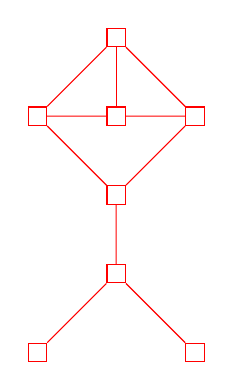
\begin{tikzpicture}[red]
\node[draw] at (0,2)  (1) {};
\node[draw] at (-1,1) (2) {};
\node[draw] at (0,1) (3) {};
\node[draw] at (1,1) (4) {};
\node[draw] at (0,0) (5) {};
\node[draw] at (0,-1) (6) {};
\node[draw] at (-1,-2) (7) {};
\node[draw] at (1,-2) (8) {};
\draw (7)--(6)--(8);
\draw (6)--(5)--(2)--(3)--(4)--(5);
\draw (2)--(1)--(4);
\draw (3)--(1);
\end{tikzpicture}
\end{document}
